
\section{Experimental Analysis}\label{sec:exp}
These benchmarks were carried out on a Dell Mobile Precision Workstation 5760 with 
Intel Xeon W-11955M (8 Core, 24MB Cache, 2.60 GHz to 5.00 GHz, 45W, vPro), 64GB DDR4 3200MHz RAM and 400GB free disk space.
\begin{figure}[!t]
	\centering
	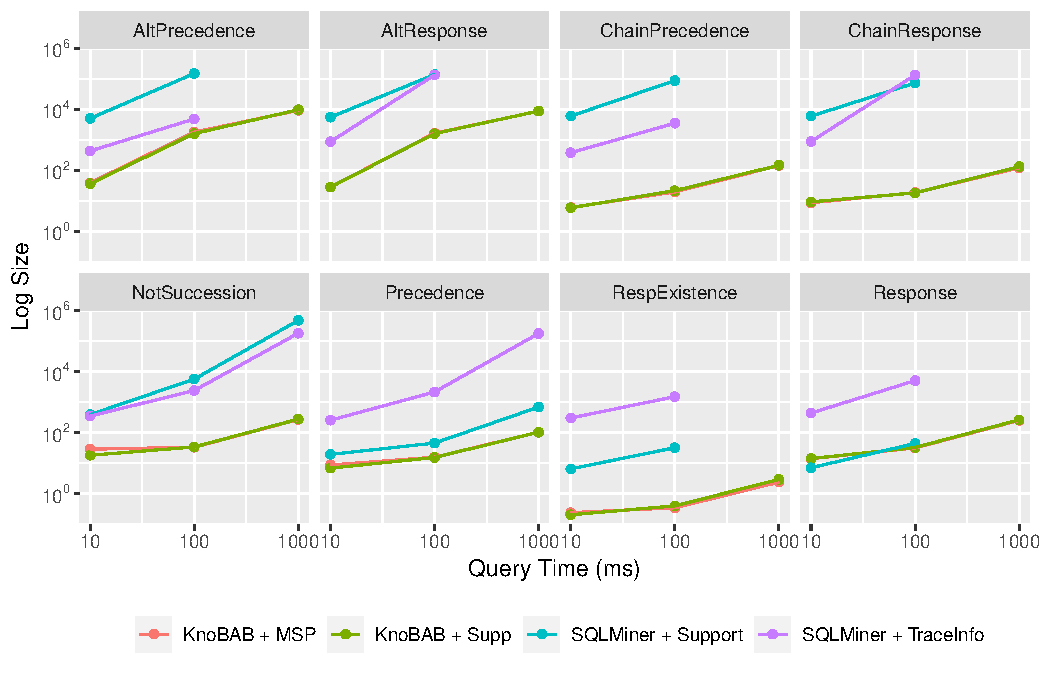
\includegraphics[width=.8\textwidth]{images/Rplot.pdf}
	\caption{KnoBAB vs SQLMiner Performance for 25  clauses with frequent activity labels with Support and Trace Information. OOM indicates Out of Memory, where $>$ 315GB of primary memory was used (causing the interruption of the computation).}\label{fig:vsSQL}
\end{figure}

\subsection{SQLMiner}\label{ssec:sqlmin}
These experiments want to test our working hypoteses related to the possibility to engineer a tailored relational database solution to run process mining through conformance checking, as well as computing conformance checking solutions. Given that the SQL provided in \cite{Schonig15} might only return the \textsc{Support} associated to each candidate declare clause (\texttt{SQLMiner+Support}), we provided the least possible changes to also associate to each candidate clause the set of all the traces satisfying it. By doing so, we extended the activation condition expressed in SQL and used \texttt{array\_aggr} provided by \textbf{PostgreSQL 13.6} to list such traces (\texttt{SQLMiner+TraceInfo}). For testing the same settings in KnoBAB, we run both Max-SAT and \textsc{Support} queries with the difference that, in our case, both of these implementations will always return per intermediate result specification the trace information satisfying each possible model clause.
We exploited the same hospital log dataset from \cite{SchonigRCJM16}: in order to test the scalability of the solutions, we randomly sampled such log with log traces with powers of ten, while guaranteeing that each downsample is always a trace subset of the samples greater than its. For each of this log, we generated a model consisting of 25 distinct declarative clauses consisting of the most frequent activity label. For SQLminer, each clause  where represented as distinct rows in \textsf{Action} associated to a specific SQL query bounded to a Declare template. KnoBAB was tested on the same resulting declare models. 

The outcome of such experiments is represented in \figurename~\ref{fig:vsSQL}, where each plot represents the running time associated to a set of different clauses: we might observe that, in the worst case scenario (\textsf{Response}), we exhibit similar query running times to SQLMiner run on PostgreSQL while, in the best case scenario, we outperform the relational database solution using SQL by at most 5 orders of magnitude. This is due to the fact that our query plan minimizes the access to the data queries and to the fact that our computation avoided explicit computations of aggregations by guaranteeing that the intermediate results are always sorted. Our solution never exceeded the 64GB of primary memory while, for some queries, SQLMiner exceeded directly the primary memory, thus proving that our solution is also memory efficient. In particular, our performances in the RespExistence can be motivated by the definition of a convenient declarative representation only accessing the \textsf{CountTable}, while the original SQL query had still to scan a \texttt{Log} table which is similar to our \texttt{ActivityTable}. This further validates that an adequate tabular representation twinned with operators tailored for. Last, running time of the Max-SAT problem and \textsc{Support} for KnoBAB exhibited similar running times, while in PostgreSQL those exhibit huge variations depending on the query-plan rewriting performed by the relational dataset. For some declarative templates, our proposed \texttt{SQLMiner+TraceInfo} formulation proved to be more efficient than \texttt{SQLMiner+Support}.


\begin{table}[!t]
	\caption{Satisfiability over the BPI 2012 Challenge}
	\centering
	\resizebox{\textwidth}{!}{\begin{tabular}{l|r|rr}
			\toprule
			\multirow{2}{*}{\textit{Conjunctive Query}} & \multicolumn{3}{c}{Query Time \textit{(ms)}} \\ 
			& \textsf{Declare Analyzer} & \textbf{KnoBAB+Conj}& \textbf{KnoBAB+Supp}\\
			\midrule
			$q_1:= \DeclareClause{Response}{A\_SUBMITTED}{\textbf{true}}{A\_ACCEPTED}{\textbf{true}}$ &  $\color{red}1.75\cdot 10^3$ & $\mathbf{1.83}\cdot \mathbf{10}^\mathbf{1}$& $2.19\cdot 10^1$\\
			$q_2:= q_1\wedge \MonoDeclareClause{Exists}{\_\_trace\_payload}{\texttt{AMOUNT\_REQ}\geq 10^3}{\geq 1}$ &  $\color{red}1.77\cdot 10^3$ & $\mathbf{2.06}\cdot \mathbf{10}^\mathbf{1}$ & $2.45\cdot 10^1$ \\
			$q_3:=q_1\wedge \MonoDeclareClause{Exists}{\_\_trace\_payload}{\texttt{AMOUNT\_REQ}< 10^3}{\geq 1}$ & $\color{red}1.62\cdot 10^3$ & $\mathbf{2.15}\cdot \mathbf{10}^\mathbf{1}$&  $2.51\cdot 10^1$\\
			$q_4:=q_1\textrm{ where }\texttt{A\_SUBMITTED.org:resource}=\texttt{A\_ACCEPTED.org:resource}$ & $\color{red}1.71\cdot 10^3$ & $\mathbf{2.43}\cdot \mathbf{10}^\mathbf{1}$& $2.77\cdot 10^1$\\
			$q_5:=q_1\textrm{ where }\texttt{A\_SUBMITTED.org:resource}\neq\texttt{A\_ACCEPTED.org:resource}$ & $\color{red}1.93\cdot 10^3$ & $\mathbf{2.59}\cdot \mathbf{10}^\mathbf{1}$& $3.01\cdot 10^1$\\
			$q_1\wedge q_2$ & $\color{red}1.81\cdot 10^3$ &  $\mathbf{2.70}\cdot \mathbf{10}^\mathbf{1}$& $3.05\cdot 10^1$\\
			$q_1\wedge q_2\wedge q_4$ & $\color{red}2.49\cdot 10^3$ & $\mathbf{2.74}\cdot \mathbf{10}^\mathbf{1}$ & $3.15\cdot 10^1$\\
			$q_1\wedge q_3\wedge q_4$ & $\color{red}2.38\cdot 10^3$ & $\mathbf{2.51}\cdot \mathbf{10}^\mathbf{1}$& $2.80\cdot 10^1$\\
			$q_1\wedge q_2\wedge q_5$ &$\color{red}2.06\cdot 10^3$  & $\mathbf{2.57}\cdot \mathbf{10}^\mathbf{1}$& $2.95\cdot 10^1$\\
			$q_1\wedge q_3\wedge q_5$ & $\color{red}2.19\cdot 10^3$ & $\mathbf{2.29}\cdot \mathbf{10}^\mathbf{1}$& $2.55\cdot 10^1$\\
			$q_1\wedge q_2\wedge q_3\wedge q_4\wedge q_5$ & $\color{red}2.90\cdot10^3$ & $\mathbf{2.66}\cdot \mathbf{10}^\mathbf{1}$ & $3.01\cdot 10^1$\\
			\bottomrule
	\end{tabular}}
\end{table}

\subsection{Declare Analyzer}\label{ssec:declan}

The benefits from the custom query plan are most obvious in the process mining stage, where a log consisting of potentially thousands of traces is tested against all combinations of clauses. However, computational gains can also be evidenced when the same querying approach is adapted to a runtime scenario, where we are querying only 1 trace against an existing model (which requires much less computation as a whole).

For $\mathcal{C}$ Declare clauses, where $\mathcal{N}$ is the data loading cost, implementations without a KB suffer, resulting in $\mathcal{O(C \cdot N)}$ complexity. With a KB, data loading is necessary only once, enhancing the complexity to $\mathcal{O(C + N)}$.

However these are computationally bottlenecked to the efficiency of these systems themselves, regardless of the optimality of the conformance checking.

\RevDel{SQL miner, due to the query structure, requires vast amounts of secondary memory for temporary caching of query computation, {much less than KnoBAB requires}.}